\documentclass[9pt,twocolumn,twoside]{osajnl}
%% Please use 11pt if submitting to AOP
% \documentclass[11pt,twocolumn,twoside]{osajnl}

\journal{ol} % Choose journal (ao, aop, josaa, josab, ol)

% See template introduction for guidance on setting shortarticle option
\setboolean{shortarticle}{true}
% true = letter / tutorial
% false = research / review article
% (depending on journal).

\title{Distribution of twin beam at 1550 nm telecom band over 26 km optical fiber}

\author[1]{Yuhong Liu, Nan Huo}
\author[1,*]{Xiaoying Li}


\affil[1]{College of Precision Instrument and Opto-electronics Engineering, Tianjin University, Key Laboratory of Optoelectronics Information Technology of Ministry of Education, Tianjin 300072, China}

\affil[*]{Corresponding author: xiaoyingli@tju.edu.cn}

%% To be edited by editor
% \dates{Compiled \today}

\ociscodes{(270.0270) Quantum Optics; (060.4370) Nonlinear optics, fibers; (190.4380) Nonlinear optics, four wave mixing}

%% To be edited by editor
% \doi{\url{http://dx.doi.org/10.1364/XX.XX.XXXXXX}}

\begin{abstract}
We experimentally measured 5.8dB intensity squeezing generated by all-fiber system and demonstrated transmission of intensity squeezing state in 26 km telecom single mode fiber while maintaining 2dB squeezing.
Our experiment shows that the long-haul transmission of intensity squeezed state does not introduce additional noise to the intensity squeezed state.
% Our result shows that the primary limit of measured squeezing is the loss of transmission fiber, which can be improved by low loss fibers.
\end{abstract}

\setboolean{displaycopyright}{true}

\begin{document}

\maketitle
%%%%%%%%%%%% Introduction %%%%%%%%%%%%%%%%%%%%%%%%%%%%%%%%%%%%%%%%%%%%%
\section{Introduction}


Creation and distribution of the continuous-variable quantum states are important for quantum communication applications, such as teleportation, dense coding and quantum key distribution\cite{braunstein_quantum_2005}.
For long distance quantum communication protocols, such as quantum key distribution and quantum teleportation, transmitting quantum state far enough while keeping its quantum property is essential.
Modern fiber communication networks are able to transmit light in telecom band with little loss, which is very promising for quantum communication.
There has been much endeavor in trying to transmit quantum states further[Satellite, Fiber, Air] and transmit quantum state with low loss fiber network is a nice solution.
%We present an all-fiber pulsed twin beams source in telecom band which is compatible with fiber telecommunication networks.
We experimentally launched twin beams generated by all fiber source into fiber telecommunication networks.
The twin beams are distributed over 26km single mode fiber (SMF) and still remain 2dB squeezing, which is the longest for continuous variable state distribution.
%The directly measured intensity difference squeezing is $R_{0}= 5.8$ dB.%, which is the best reported in fiber system.
%Besides, twin beams generated in telecom band by fiber system are compatible with conventional single mode fiber (SMF). %, and suffers way much less coupling loss into SMF. % (around 4\% splicing loss and can be less if the fibers are properly tapered before splicing) than those generated by crystals and atom systems.%degrades the squeezing by introducing new vacuum.
%The twin beams are transmitted by individual SMFs for long distance to test its vulnerability to transmission loss and other noise.
%After distribution in SMF for 4, 10, 16 and 26km, the measured normalized noise power is still 2dB below shot noise limit defined by detected intensity.
Comparing the experimental results with the theoretically expected values, we find that the only limitation for further propagation is the fiber transmission loss. Pulsed nature of our twin beams source provide further advantages over continuous wave squeezing which suffers from stimulated Brillouin scattering\cite{feng_distribution_2017}.
%, which can be improved with the help of low loss fiber.
%Thus, our twin beam source has great potential in quantum information and quantum cryptology.



%Intensity squeezing is a useful tool for quantum information, quantum metrology and some other things that I don't know.
%In experiment that xxxxx, it's important to transmit quantum state far enough while keeping its quantum property.


% basic results
In this letter, we present a pulsed twin beam source in telecom band via Stimulated Four Wave Mixing (FWM) in Dispersion Shifted Fiber (DSF) and transmit it by two Single Mode Fiber (SMF). The initial directly measured intensity directly difference squeezing is $R_{0}= 6 dB$, which is the best reported in fiber system. Besides, twin beams generated in telecom band by fiber system are compatible with conventional SMF, and suffers less coupling loss, which is generally inevitable for those generated by crystals and atom systems.%degrades the squeezing by introducing new vacuum.

We managed to lunch the twin beams into individual SMF.
After propagating in SMF for 10km, the measured normalized noise power is still 2dB below shot noise limit defined by detected intensity. Comparing to theoretical prediction, the only limitation for further propagation is the fiber transmission loss, which can be improved with the help of low loss fiber. Thus, our twin beam source has great potential in quantum information and quantum cryptology.

\section{Theory}

Intensity difference squeezing of twin beam is defined as the ratio between intensity difference noise of twin beams and SNL at identical intensity on detectors. When FOPA is injected with coherent state, directly measured intensity difference between output beams of FOPA possess less fluctuation than classical SNL. This method is called self homodyne detection[????] and can figures out how much entanglement exists between twin beams generated.
%%
According to four wave mixing theory in fiber\cite{guo13}[???], FOPA can be depicted by Bogoliubov transformation:
\begin{equation}
\begin{array}{c}
\hat b_s = G{\hat a_s} + g\hat a_i^\dag ,   
\hat b_i = G{\hat a_i} + g\hat a_s^\dag 
\end{array}
\end{equation}
$\hat b_s$ ($\hat b_i$)is output operator of signal(idler) field, $\hat a_s$ ($\hat a_i$)is input operator of signal(idler) field, G and g satisfies the relation $G^2-g^2=1$. They are gain factor of FOPA and are related to pump power and nonlinear coefficient of DSF.
Ideally the twin beams generated from a FOPA with power gain $G$ and $g$ possess intensity difference squeezing:
\begin{equation}
{R_0} = \frac{
{\left\langle {\Delta {{({I_s} - {I_i})}^2}} \right\rangle }}
{{\left\langle {\Delta {I_s}^2} \right\rangle  + \left\langle {\Delta {I_i}^2} \right\rangle }} = \frac{1}{{({G^2} + {g^2})}}
\label{eq:R0}
\end{equation}
$I_s$ ($I_i$) is the intensity detected in signal (idler) channel. $\Delta{I_s}^2+\Delta{I_i}^2$ defines shot noise limit (SNL). When transmission and detection loss exist in experiment system, $R$ diminishes as the total loss get larger.
After series of calculation, when the total quantum efficiency of signal beam is $\eta_s$, the maximal measurable intensity difference squeezing $R_{meas}$ is:
\begin{equation}
R_{meas}=R_0(1-\eta_s)+\eta_s
\label{eq:loss}
\end{equation}see supplementary material for more detailed derivation of influence induced squeezing drop.
This relations defines the upper limit of quantum resource left after a certain amount of loss.



\section{Setup}

\begin{figure}[htbp]
\centering
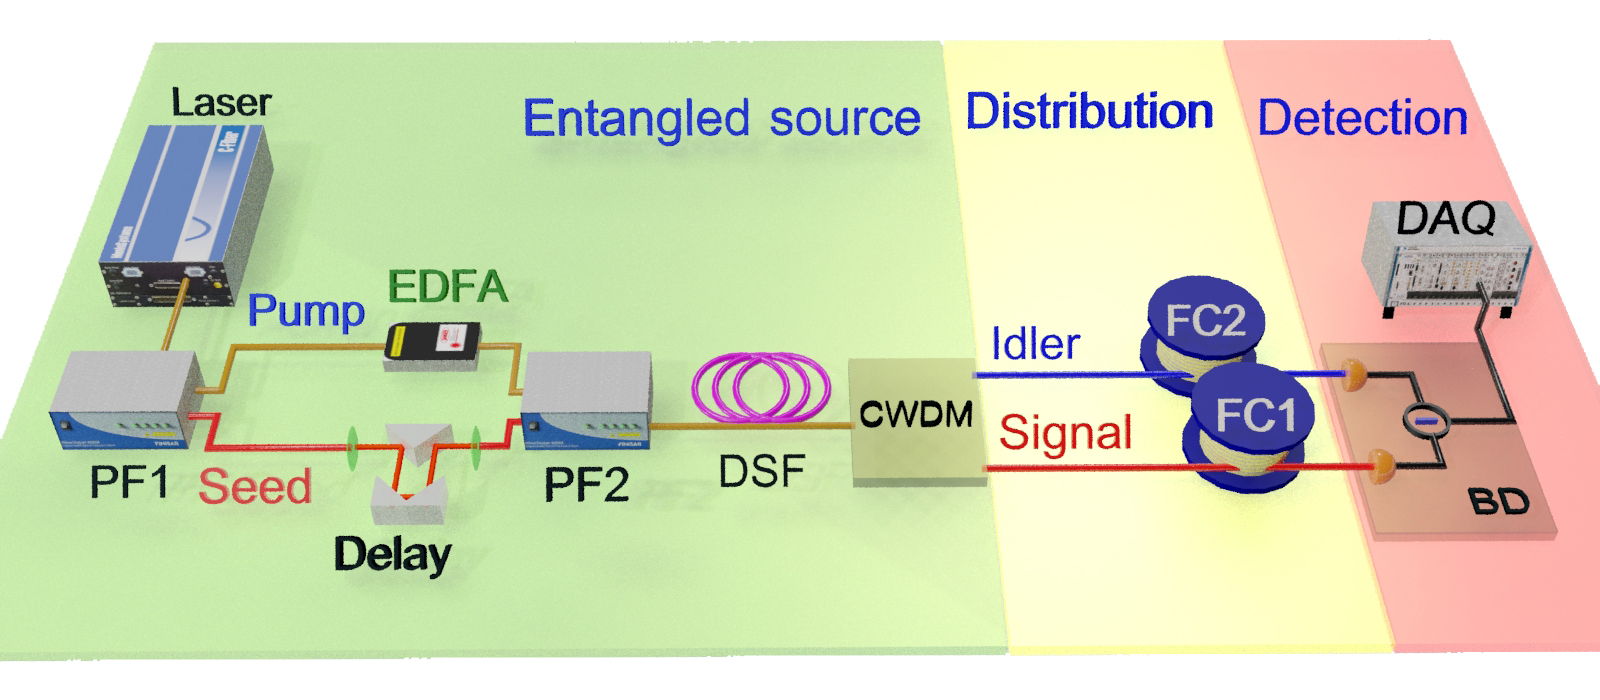
\includegraphics[width=\linewidth]{fig1_3d_2.jpg}
\caption{Experiment setup.
PF1-2, programmable optical filter;
EDFA, erbium-doped fiber amplifier;
Delay, mechanical delay line;
DSF, dispersion shifted fiber;
CWDM, coarse wavelength division multiplexers;
FC1-2, fiber coil;
BD, balanced detector;
DAQ, data acquisition system}
\label{fig_setup}

\end{figure}

\subsection{system details}
The experiment setup is shown in Fig. \ref{fig_setup}.
The non-degenerate twin beams are generated from a pulse pumped fiber optical parametric amplifier (FOPA) utilizing four wave mixing effect between strong pump and week seed injection via \(\chi^{(3)} \) nonlinear interaction in 300 m DSF fiber.
The zero dispersion wavelength of DSF is 1548.5 nm when cooled at 77 k by liquid nitrogen, which reduces additional raman noise in generated twin beams \cite{guo12}.
The Zero Dispersion Wavelength (ZDW) of DSF is 1552.6 at room temperature and shifts to 1548.5 nm when cooled at 77k by liquid nitrogen, which improves the quality of generated twin beam \cite{guo12}.

%% filter
For simplicity of narration, we denote the beam in shorter injecting wavelength signal and the conjugate beam in longer wavelength as idler.
The pump and seed are filtered separately from a mode-locked laser by Programable Filter (PF1), and the center wavelength and bandwidth of pump (seed) are 1549.5 nm (1533 nm) and 0.7 nm (1.5 nm) respectively.
After PF1, the filtered pump is further amplified by Erbium-doped Fiber Amplifier (EDFA) to meet the required power while the seed is delayed by a mechanical delay-line so as to keep overlapped with pump in DSF.
The amplified pump and seed is combined at the PF2 and feed into DSF where twin beams are generated via FWM.
Besides, PF2 also filter out ASE from EDFA and compensate dispersion from previous fiber system, which helps to increase the gain of OPA.
After amplification in DSF, twin beams are generated and separated by 15nm bandwidth Coarse Wavelength Division Multiplexer (CWDM), which has 90\% and 86\% transmission efficiency in signal (centered at 1531nm) and idler channel (centered at 1571nm)  respectively with DSF-SMF splicing loss at the output of DSF(4\%) and SMF-SMF splicing loss between CWDM filters(<1\%) included.
%% transmission
The separated twin beam is transmitted individually by single mode Fiber Coil FC1 and FC2, which has equal length so as to simplify the detection system.
The SMF used has typical 0.2dB/km transmission loss and the length is set to 0, 2, 5, 8 and 13 km, corresponding to distribution of entangled source by 0, 4, 10, 16, 26 km respectively, so as to demonstrate the potential of twin beam in long haul quantum resource distribution.

%% detection and electronics
The signal and idler of twin are detected by a Balanced Detector (BD) directly.
The BD used in our experiment is modified Thorlabs PDB450C, with detectors replaced by high quantum efficiency (96\% with coupling efficiency included) InGaAs Pin detectors from Laser Components.
The 3dB bandwidth of BD is 0.4MHz. When input power is 15 uW per detector, the measured SNL is 16dB higher than electronic noise.
The RF signal output, filtered by 1.9MHz low pass anti-aliasing filter and further amplified by commercial RF amplifiers, and DC monitors of BD is sent to DAQ system, which is an integrated system including spectrum analyzer and local intensity monitor.
The noise power is analyzed by digitally filtering out signal from 180kHz with 220kHz.
The SNL of BD is calibrated by coherent light at different input power in prior to other measurement.
When measuring intensity difference, the signal noise power is compared with SNL at same intensity in realtime, which helps to make the experiment result free from power drifting and fluctuation.


The intensity of twin beams generated from FOPA are naturally unbalanced due to the relation $G^2-g^2=1$, were $G^2$ and $g^2$ are signal and idler power gain. 
Besides, transmission loss in different channel and Raman amplification effect, which provide addition gain and noise together in longer wavelength, also make this problem more sophisticated.
In previous works\cite{guo12}, when the inject wavelength is longer than pump wavelength, the inject signal obtain much more power gain, and thus we had to attenuate the inject signal a lot(>10\%), which is undesirable. 
Here we change the inject wavelength to shorter wavelength, the power gain in idler channel is almost identical with signal field, which means we only need to attenuate idler field slightly(1-2\%).



\section{Results}

We first measure the twin beam directly after the generation.
Fig. \ref{fig2_OPA}(a) shows the measured intensity difference squeezing at different OPA gain with the insert showing the gain of OPA at different pump power.
It can be seen that the maximum squeezing reached in our experiment is 5.8dB when the power gain of OPA is arond 30.
The measured squeezing decrease slightly when the gain of OPA increase further, which is probably caused by raman effect who introduce additional noise to both signal and idler field.

In fig. \ref{fig2_OPA}(b) shows the best noise reduction result read on the DAQ system when pump power is 1.4 mW and intensity of signal and idler field is both around 15 uW. The intensity difference noised after cancelation of electronic noise and normalized to SNL is shown by line(2). Line(1) is recorded corresponding SNL with identical intensity. It's obvious to see more than 5.8 dB noise reduction from SNL.
%Even though, the best result cancels out Electronic Noise (EN) shown by line3, the influence over uncorrected squeezing is no more than a slight change.
According to eq.\ref{eq:loss}, the normalized intensity noise generated from OPA is more than 8.5 dB after efficiency correction%
%(90\% for signal field and 85 for idler field). the QE of Detector is around 96%	
(86\% for signal field and 81 for idler field).	
Further more, this twin beam source is obviously broadband squeezed as the squeezing spread through the whole measured frequency span until limited by electronic filtering, which can be overcome by changing the electronics of BD.

\begin{figure}[htbp]
\centering
%\includegraphics[width=7cm]{Gain_and_sqz_vertical.jpg}%{Gain_and_sqz.jpg}
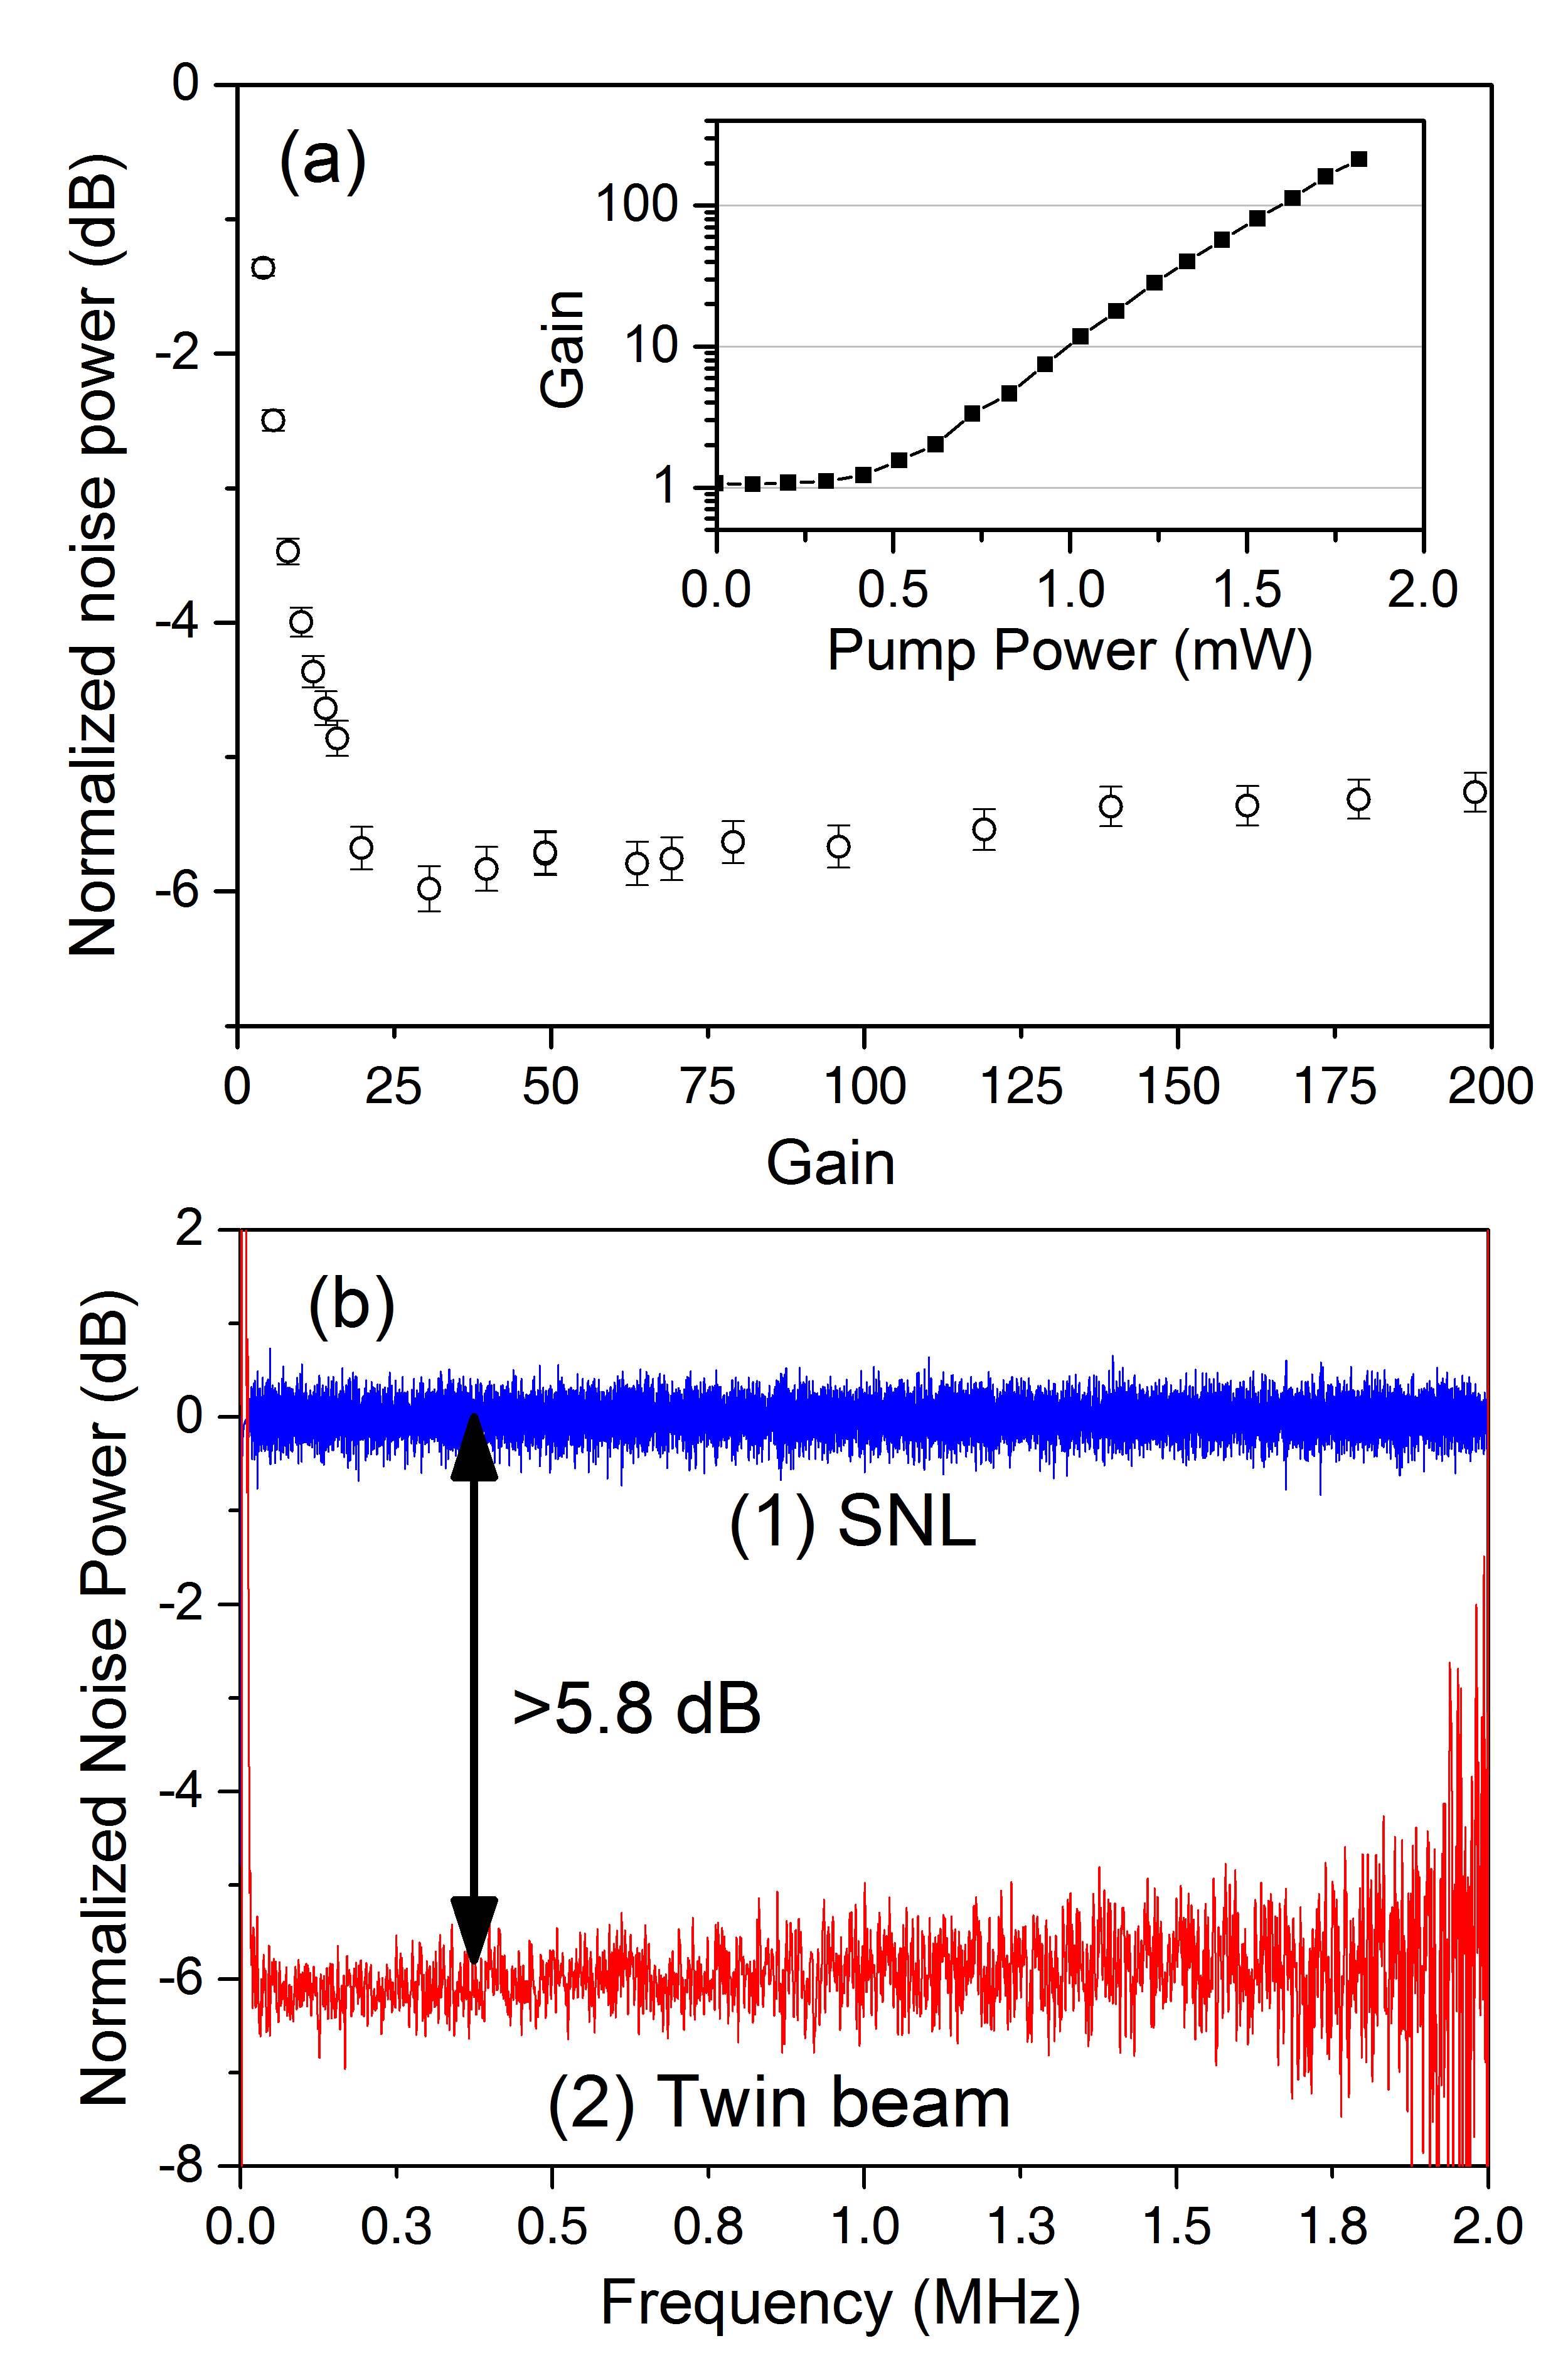
\includegraphics[width=7cm]{Gain_and_sqz_vertical_EN_cor.jpg}%{Gain_and_sqz.jpg}
\caption{Performance of intensity difference squeezing. (a) Intensity difference squeezing at different power gain of FOPA. Insert is the  power gain of FOPA at different pump power. (b) Maximum intensity difference squeezing measured. Line (1), shot noise limit for intensity measured by line(2). Line (2) is the normalized intensity difference noise with electronic noise of detection system cancelled.}
\label{fig2_OPA}
\end{figure}

\begin{figure}[htbp]
\centering
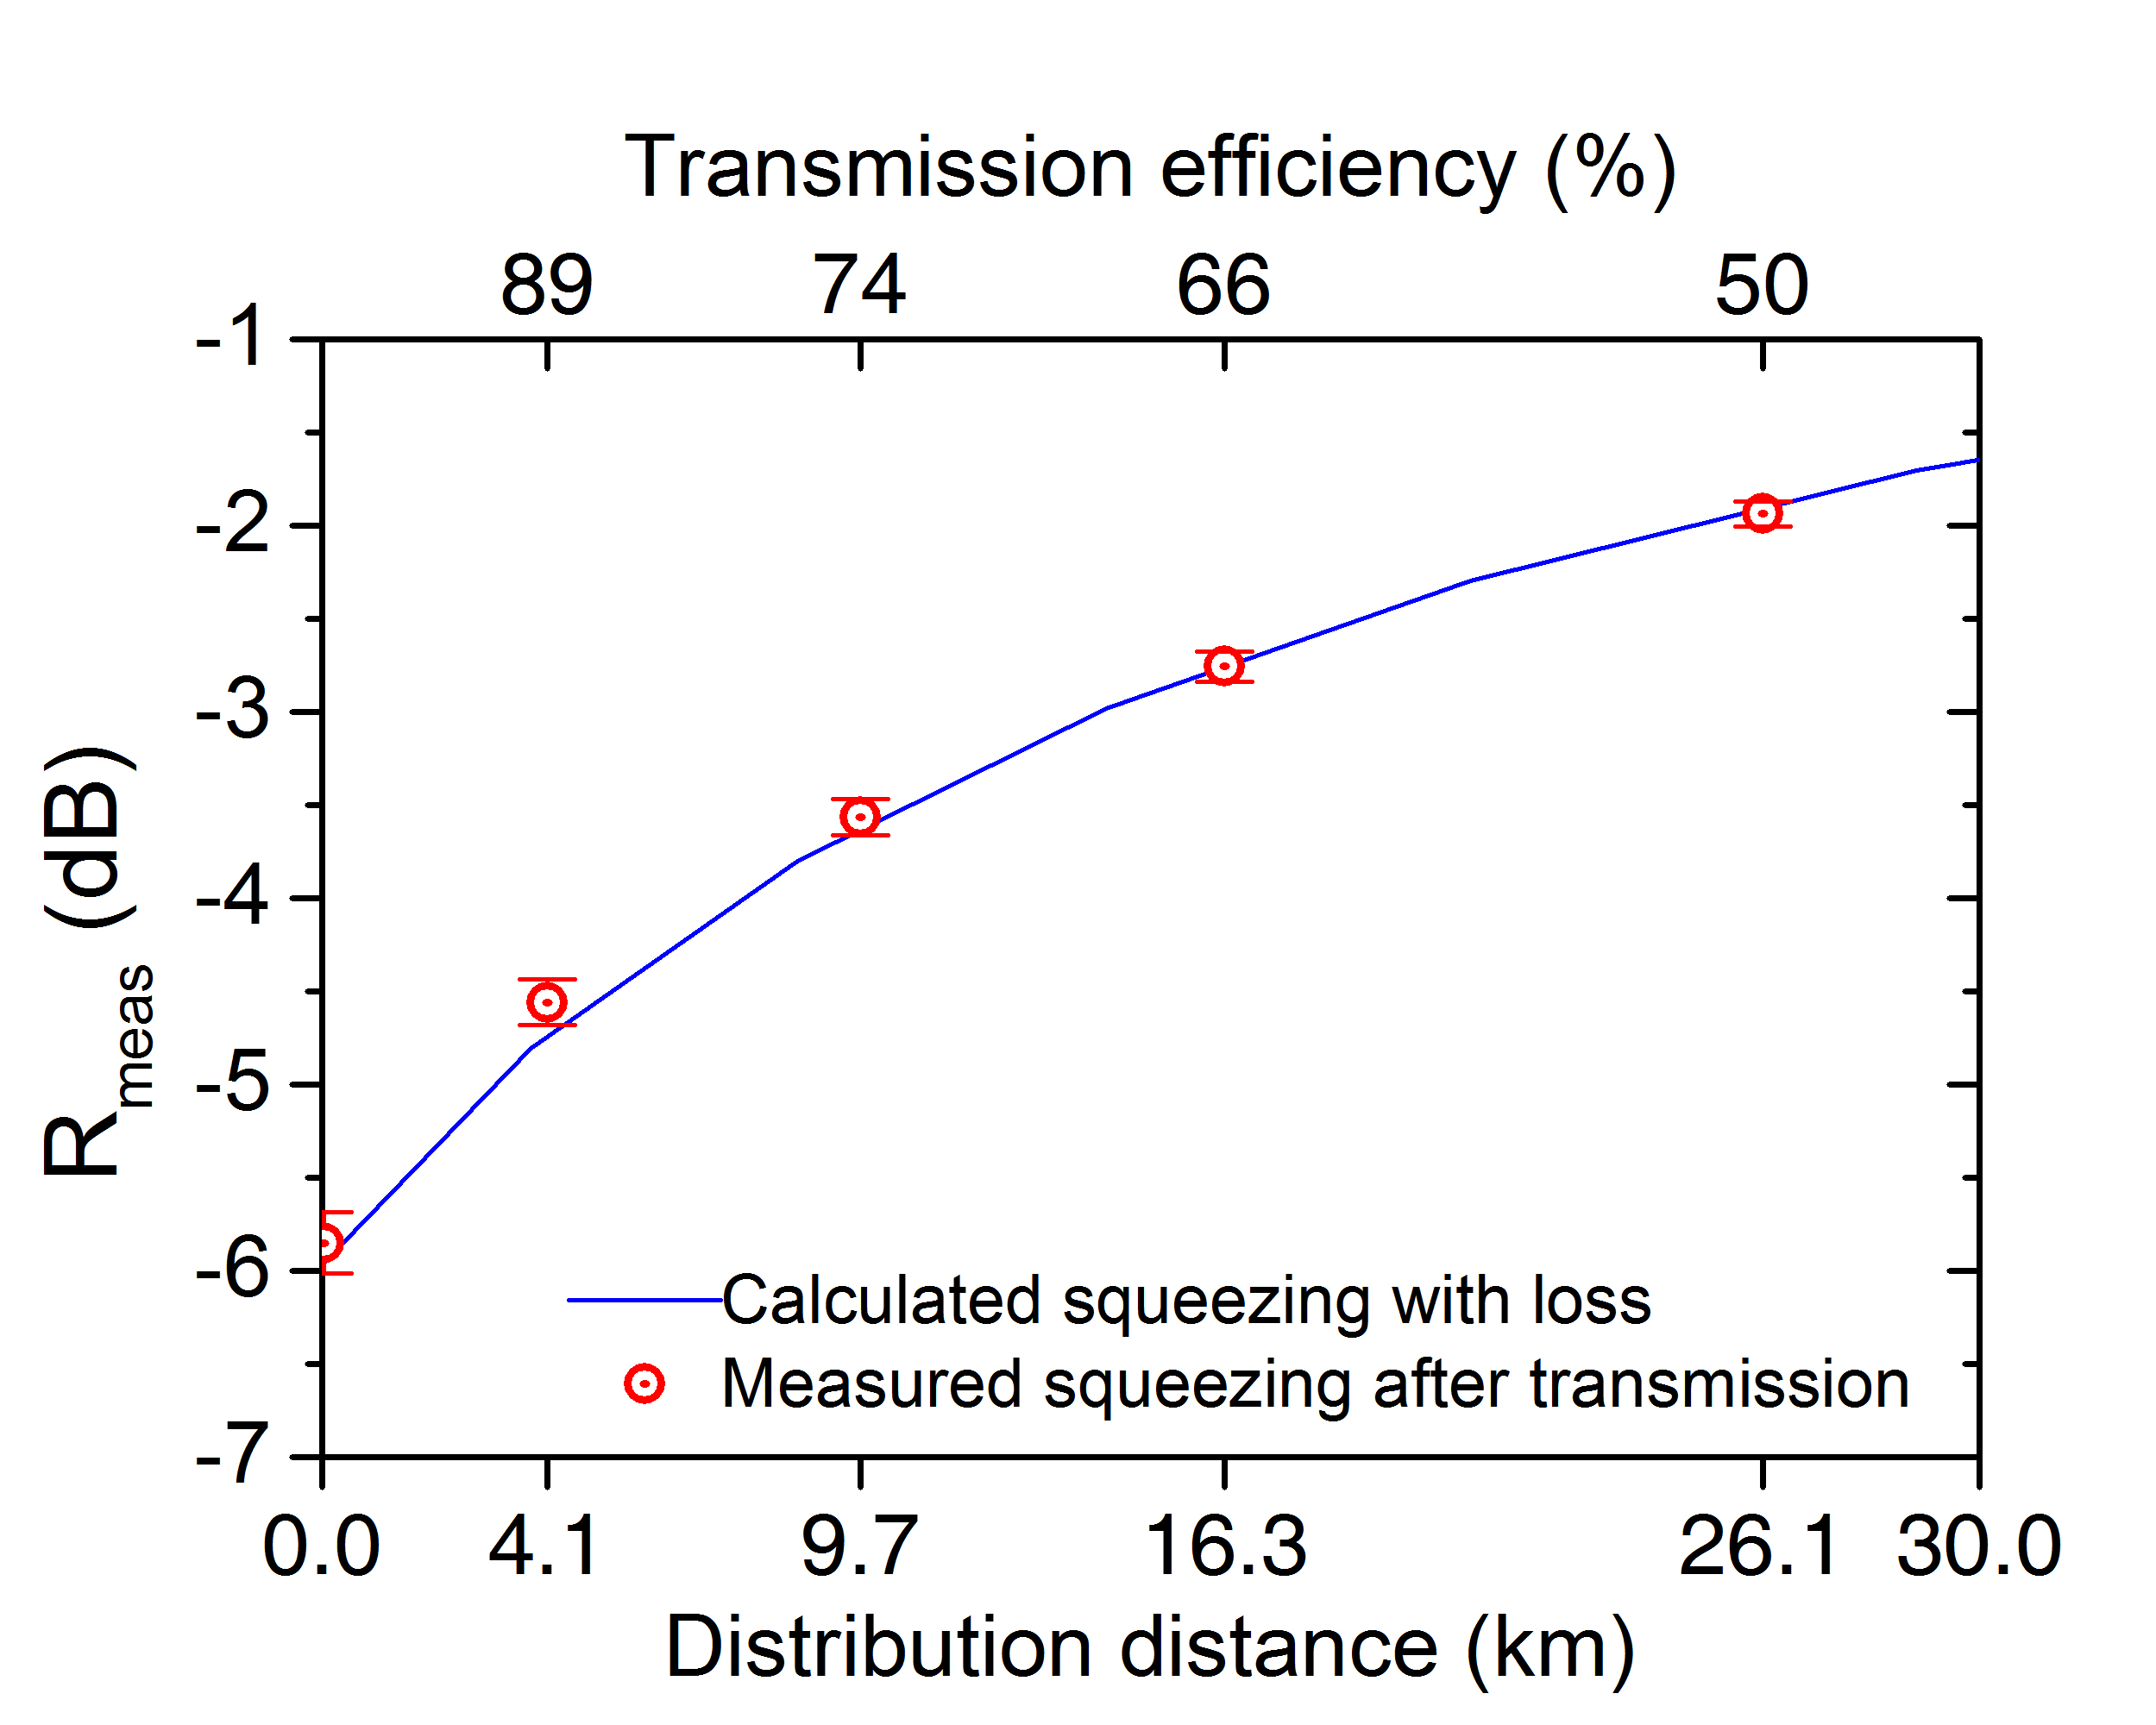
\includegraphics[width=7cm]{Sqz_vs_Length_dB_color.jpg}
\caption{Measurable intensity difference squeezing at different transmission loss}
\label{fig_loss}
\end{figure}
\subsection{transmission loss}
Based on eq.\ref{eq:loss}, we calculated the normalized intensity noise at different transmission loss caused by transmission in SMF and plotted by blue line in fig. \ref{fig_loss}. The top axis is the signal field detection efficiency, and the bottom axis is the length of SMF that cause same amount of transmission loss. As shown in the figure, intensity squeezing can endure a pretty long SMF transmission and keep more than 2dB squeezing after distributing the twin beam by 26km, which are realized by 13km SMF on signal and idler channel respectively.

After analysis above, we launch the generated twin beams into two SMFs individually, the output from two SMFs are detected by BD shown in fig. \ref{fig_setup}.
After different length of fiber, the attenuation caused by fiber transmission loss makes the measured intensity squeezing degrade accordingly.
The relation between fiber length and intensity difference squeezing $R_{meas}$ is plot as red dots in fig. \ref{fig_loss}.
Comparing to theoretical prediction plot as blue line, the experiment result agrees well with the equation (\ref{eq:loss}).
The result indicates that there is no additional noise introduced during distribution over SMF except for transmission loss, which can be improved by ultra low loss fibers with 0.15 dB/km transmission loss [???find someone].

\subsection{intensity influence}
We also explore how the intensity of twin beams influence the experiment result and try to figure out RIN noise introduced by pump and inject power fluctuation.



\section{Conclusion}
In conclusion, we experimentally built an all fiber twin beam source that possess 5.8 dB direct measurable intensity squeezing(8.5dB after efficiency correction).
The generated twin beam is distributed by 26 km and still remains 2 db squeezing, which fits theoretical prediction well and no other unwanted noise are introduced.
This all fiber twin beams source is compatible with conventional fiber communication systems and shows great potential in quantum conmmucation and long distance quantum metrology.


\section{Funding Information}


\section{References}

% Bibliography
\bibliography{10km_sqeezing}
\bibliographyfullrefs{10km_sqeezing}
\ifthenelse{\equal{\journalref}{aop}}{%

\section*{Author Biographies}
\begingroup
\setlength\intextsep{0pt}
\begin{minipage}[t][6.3cm][t]{1.0\textwidth} % Adjust height [6.3cm] as required for separation of bio photos.
  \begin{wrapfigure}{L}{0.25\textwidth}
    
\includegraphics[width=0.25\textwidth]{john_smith.eps}
  \end{wrapfigure}
  \noindent
  {\bfseries John Smith} received his BSc (Mathematics) in 2000 from The University of Maryland. His research interests include lasers and optics.
\end{minipage}
\begin{minipage}{1.0\textwidth}
  \begin{wrapfigure}{L}{0.25\textwidth}
    
\includegraphics[width=0.25\textwidth]{alice_smith.eps}
  \end{wrapfigure}
  \noindent
  {\bfseries Alice Smith} also received her BSc (Mathematics) in 2000 from The University of Maryland. Her research interests also include lasers and optics.
\end{minipage}
\endgroup
}{}

\end{document} 